In this section, we prove the theorem described above.

We first make explicit how we formalize language processing for proving the theorem.

\paragraph{Language as a Stochastic Process}
We represent language as a stochastic process:
We formalize a language as a probabilistic sequence of words $\dots w_{-2} w_{-1} w_0 w_{1} w_{2} \dots$, extending indefinitely both into the past and into the future.
The symbols $x_i$ belong to a common set, representing the words of the language.\footnote{Could also be phonemes, sentences, ..., any other kind of unit.}

We model the sequence as a probabilistic sequence; that is, given a context $w_{<t}$, the next word is distributed according to a distribution $p(w_t|w_{<t})$.

The assumption of infinite length is for mathematical convenience and does not affect the substance of our results:
As we restrict our attention to the processing of individual sentences, which have finite length, we will actually not make use of long-range and infinite contexts.

We make the assumption that this process is \emph{stationary}.
Formally, this means that the conditional distribution $P(w_t|w_{<t})$ does not depend on $t$, it only depends on the actual sequence $w_{<t}$.
Informally, this says that the process has no `internal clock', and that the statistical rules of the language do not change at the timescale we are interested in.
In reality, the statistical rules of language do change: They change as language changes over generations, and they also change between different situations -- e.g., depending on the interlocutor at a given point in time.
Given that we are interested in memory needs in the processing of \emph{individual sentences}, at a timescale of seconds or minutes, stationarity seems to be a reasonable assumption to make.





\begin{figure}
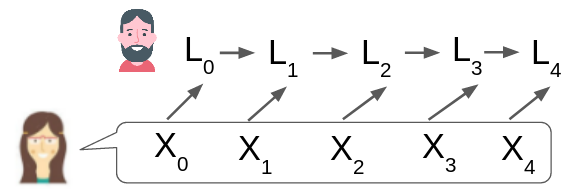
\includegraphics[width=0.45\textwidth]{figures/markov-condition.png}
	\caption{Illustration of (\ref{eq:listener-markov}). As the utterance unfolds, the listener maintains a memory state. After receiving word $w_t$, the listener computes their new memory state $L_t$ based on the previous memory state $L_{t-1}$ and the new word $w_t$.}\label{fig:listener-markov}
\end{figure}


\paragraph{Listener's Memory}
We now analyze memory from the perspective of the listener, who needs to maintain information about the past to predict the future.
As the speaker's utterance unfolds, the listener maintains a memory state $L_t$.



There are no assumptions about the memory architecture and the nature of its computations.
We only make a basic assumption about the flow of information (Figure~\ref{fig:listener-markov}):
At a given point in time, the listener's memory state $L_t$ is determined by the last word $w_t$, and the prior memory state $L_{t-1}$.
As a consequence, $L_t$ contains no information about the process beyond what is contained in the last word observed $w_{t-1}$ and in the memory state before that word was observed $L_{t-1}$.
This is formalized as a statement about conditional probabilities:
	\begin{equation}\label{eq:listener-markov}
		p(L_1| (w_{t})_{t \in \mathbb{Z}}, L_0)   = p((w_{t})_{t \in \mathbb{Z}} | L_0, w_1)
%p((w_{t})_t| L_0, L_1, w_1)   = p((w_{t})_t| L_0, w_1)
	\end{equation}
This says that $L_1$ contains no information about the utterances beyond what is contained in $L_0$ and $w_1$.	
As a consequence, the listener has no knowledge of the speaker's state beyond the information provided in their prior communication.
This is a simplification, as the listener could obtain information about the speaker from other sources, such as their common environment (weather, ...).
For the study of memory in sentence processing, this seems fair. Discuss this more.

%
%First, we assume that the listener's internal state cannot depend on the future beyond its dependency on the past.
%Formally: 
%\begin{equation}\label{eq:listener-markov-1}
%L_t \bot w_{>t} | w_{\leq t}
%\end{equation}
%This means that the listener has no access to the speaker's state beyond what the speaker has already uttered.
%
%Second, we assume that $L_t$ contains no information about the past beyond what is contained in $w_{t-1}$ and $L_{t-1}$:
%\begin{equation}\label{eq:listener-markov-2}
%L_t \bot w_{<t} | w_{t-1}, L_{t-1}
%\end{equation}
%This means that any information about the past in $L_t$ has to be contained in $L_{t-1}$ -- formalizing the idea that a listener can only remember aspects of the past by keeping them in memory, and that memories of the past cannot `spontaneously' form later in the future.

%The listener can trade off memory and future surprisal:
%A listener who chooses to store less memory will exerience higher surprisal in the future.
%A listener can achieve minimal surprisal -- that is, the lowest average surprisal that any model could achieve by predicting the future from the past -- if and only if $L_t$ contains all predictive information about the future that is contained in the past.

%We now describe the memory-surprisal tradeoff. will describe this tradeoff, and show that listener memory is linked to locality in a way similar to speaker memory.
%Consider a listener who uses $J$ bits of memory on average.
%What can we say about the listener's surprisal?


\begin{thm}\label{prop:suboptimal}
	Let $T$ be any positive integer ($T \in \{1, 2, 3, ...\}$), and consider a listener using at most
	\begin{equation}\label{eq:memory}
		\sum_{t=1}^T t I_t
	\end{equation}
bits of memory on average.
Then this listener will incur surprisal at least
	$$H[w_t|w_{<t}] + \sum_{t > T} I_t$$
	on average.
\end{thm}
The proof is given in the appendix (REF).




\subsection{Proof of the Theorem}



%\begin{proof}
	We denote the listener's memory state at time $t$, after hearing $w_{<t} = ... w_{t-2} w_{t-1}$ by $L_t$.
	The average number of bits required to encode this state is $\operatorname{H}[L_t]$, which by assumption is at most $\sum_{t=1}^T t I_t$.
	As the listener's predictions are made on the basis of her memory state, her average surprisal is at least $\operatorname{H}[w_t | L_t]$.
	The difference between the listener's surprisal and optimal surprisal is thus at least $\operatorname{H}[w_t | L_t] - \operatorname{H}[w_t | w_{<t}]$.
By the assumption of stationarity, we can rewrite this expression as
\begin{align*}
	\operatorname{H}[w_t | L_t] - \operatorname{H}[w_t | w_{<t}] &=  \frac{1}{T} \sum_{t=1}^{T} \left(\operatorname{H}[w_t | L_t] - \operatorname{H}[w_t | w_{<t}]\right) 
\end{align*}
	\begin{lemma}
For any $t$, the following inequality holds:
%	$$H[w_t | L_t] \geq H[w_t| w_{t-1}, L_{t-1}] \geq ... \geq H[w_t|w_{1 \dots t-1}, L_0]$$
	\begin{equation}
%H[w_t | L_t] \geq H[w_t| w_{t-1}, L_{t-1}] \geq ... \geq H[w_t|w_{1 \dots t-1}, L_0]
H[w_t | L_t] \geq H[w_t|w_{1 \dots t-1}, L_0]
		\end{equation}
	\end{lemma}
	\begin{proof}[Proof of the Lemma]

By Equation~\ref{eq:listener-markov}:
	\begin{equation}
p((w_{t})_t| L_0, L_1, w_1)   = p((w_{t})_t| L_0, w_1)
	\end{equation}
we have
	\begin{align*}
p(w_t|w_{<1}, L_0, L_1, w_1, w_{2 \dots t-1}) = p(w_t|w_{<1}, L_0,  w_1, w_{2 \dots t-1}) \\
p(w_{<1}| L_0, L_1, w_1, w_{2 \dots t-1})   = p(w_{<1}| L_0, w_1, w_{2 \dots t-1})
	\end{align*}
Therefore
\begin{align*}
p(w_t|L_0, w_1, w_{2 \dots t-1}; L_1, w_{2 \dots t-1}) & = p(w_t|L_0, L_1, w_1, w_{2 \dots t-1}) \\
& = \sum_{w_{<1}} p(w_t|w_{<1}, L_0, L_1, w_1, w_{2 \dots t-1}) p(w_{<1}| L_0, L_1, w_1, w_{2 \dots t-1}) \\
&= \sum_{w_{<1}} p(w_t|w_{<1}, L_0,  w_1, w_{2 \dots t-1}) p(w_{<1}| L_0, w_1, w_{2 \dots t-1}) \\
&= p(w_t|L_0,  w_1, w_{2 \dots t-1}) 
\end{align*}
Thus we have a Markov chain
\begin{equation}
(w_t) \rightarrow (L_0, w_1, w_{2 \dots t-1})   \rightarrow   (L_1, w_{2 \dots t-1})
\end{equation}
Thus, by the Data Processing Inequality,
	\begin{equation}
H[w_t| w_{2 \dots t-1}, L_{1}] \geq H[w_t|w_{1 \dots t-1}, L_0]
	\end{equation}

Finally, iteratively applying this inequality, we get:
		\begin{align*}
		H[w_t | L_t] \geq H[w_t| w_{t-1}, L_{t-1}] \geq H[w_t| w_{t-2, t-1}, L_{t-2}] \geq ... \geq H[w_t|w_{1 \dots t-1}, L_0]
		\end{align*}

	\end{proof}
	
	% = \int dw_{<1} p(w_t|w_{<1}, w_1, w_{2 \dots t-1})  = \int dw_{<1} p(w_t|L_0, w_{<1}, w_1, w_{2 \dots t-1}) = p(w_t|L_0, w_1, w_{2 \dots t-1}) $

%	$p(w_t|L_0, w_1, w_{2 \dots t-1}; L_1, w_{2 \dots t-1}) = p(w_t|L_0, L_1, w_1, w_{2 \dots t-1}) = \int dw_{<1} p(w_t|w_{<1}, L_0, L_1, w_1, w_{2 \dots t-1}) = \int dw_{<1} p(w_t|w_{<1}, w_1, w_{2 \dots t-1})  = \int dw_{<1} p(w_t|L_0, w_{<1}, w_1, w_{2 \dots t-1}) = p(w_t|L_0, w_1, w_{2 \dots t-1}) $

	Plugging this inequality into the equality above:
\begin{align*}
	\operatorname{H}[w_t | L_t] - \operatorname{H}[w_t | w_{<t}]& \geq \frac{1}{T} \sum_{t=1}^T ( \operatorname{H}[w_t|w_{1\dots t-1}, L_0] - \operatorname{H}[w_t | w_{1\dots t-1}, w_{\leq 0}]  )    \\
	& = \frac{1}{T} \left(\operatorname{H}[w_{1\dots T} | L_0] - \operatorname{H}[w_{1\dots T} | w_{\leq 0}]\right)  \\
	& = \frac{1}{T} \left(I[w_{1\dots T}|w_{\leq 0}] - I[w_{1\dots T}|L_0]\right) 
\end{align*}
	The first term $I[w_{1\dots T}|w_{\leq 0}]$ can be rewritten in terms of $I_t$:
	\begin{align*}
		I[w_{1\dots T}|w_{\leq 0}] &= \sum_{i=1}^T \sum_{j=-1}^{-\infty} I[w_i, w_j | w_{j+1}...w_{i-1}] = \sum_{t=1}^T t I_t + T \sum_{t > T} I_t
	\end{align*}
	Therefore
\begin{align*}
	\operatorname{H}[w_t | L_t] - \operatorname{H}[w_t | w_{<t}]& \geq \frac{1}{T} \left(\sum_{t=1}^T t I_t + T \sum_{t > T} I_t - I[w_{1\dots T}|L_0]\right) 
	%	&= \frac{1}{T} \left(\sum_{t=1}^\infty t I_t - \sum_{t > T}  (T-t) I_t- I[w_{1\dots T}|L_0]\right) \\
\end{align*}
	$I[w_{1\dots T}|L_0]$ is at most $\operatorname{H}[L_0]$, which is at most $\sum_{t=1}^T t I_t$ by assumption. Thus, the expression above is bounded by
	\begin{align*}
	\operatorname{H}[w_t | L_t] - \operatorname{H}[w_t | w_{<t}]& \geq \frac{1}{T} \left(\sum_{t=1}^T t I_t + T \sum_{t > T} I_t - \sum_{t=1}^T t I_t\right) \\
		&= \sum_{t > T} I_t
\end{align*}
	Rearranging shows that the listener's surprisal is at least $\operatorname{H}[w_t|L_t] \geq \operatorname{H}[w_t | w_{<t}] + \sum_{t > T} I_t$, as claimed.
%\end{proof}


Justify linear interpolation: The curve is convex, which is shown by `time-sharing': Use one code $\lambda$ fraction of times, and the other code $1-\lambda$ fraction of times.

